
\documentclass[a4paper,12pt]{scrbook}
\usepackage{amsmath,amssymb,amsthm}
\usepackage{fancyvrb}
\usepackage{parskip}
\usepackage{lastpage}
\usepackage{verbatim,boxedminipage,enumitem}
\usepackage{ifthen}
\usepackage{color,graphicx}
\usepackage{pgf}
\usepackage{longtable}
\usepackage{upquote}
%\usepackage[all]{xy}
\usepackage{tobiShell}
\usepackage{tikz}
\usetikzlibrary{automata}
\usetikzlibrary{arrows}
\usepackage{pgf,pgfarrows,pgfnodes}
\usepackage{pgfplots}
\usepackage{circuitikz}
\usetikzlibrary{circuits}
\usetikzlibrary{circuits.logic.US}
\usepackage{mymath}
\usepackage{python}
%------------------------------------------------------------------
% Verbatim for console window - single line frame, no line numbers
%------------------------------------------------------------------
\DefineVerbatimEnvironment%
 {console}{Verbatim}
 {frame=single}

%--------------------------------------------------------
% Remove the vertical spacing before and after Verbatim.
%--------------------------------------------------------
\usepackage{atbeginend}
\BeforeBegin{console}{\mbox{}\\ \begin{minipage}{\textwidth}\vspace{3pt}}
\AfterEnd{console}{\vspace{4pt} \end{minipage} \\ }

\begin{document}
\thispagestyle{empty}

\begin{center}
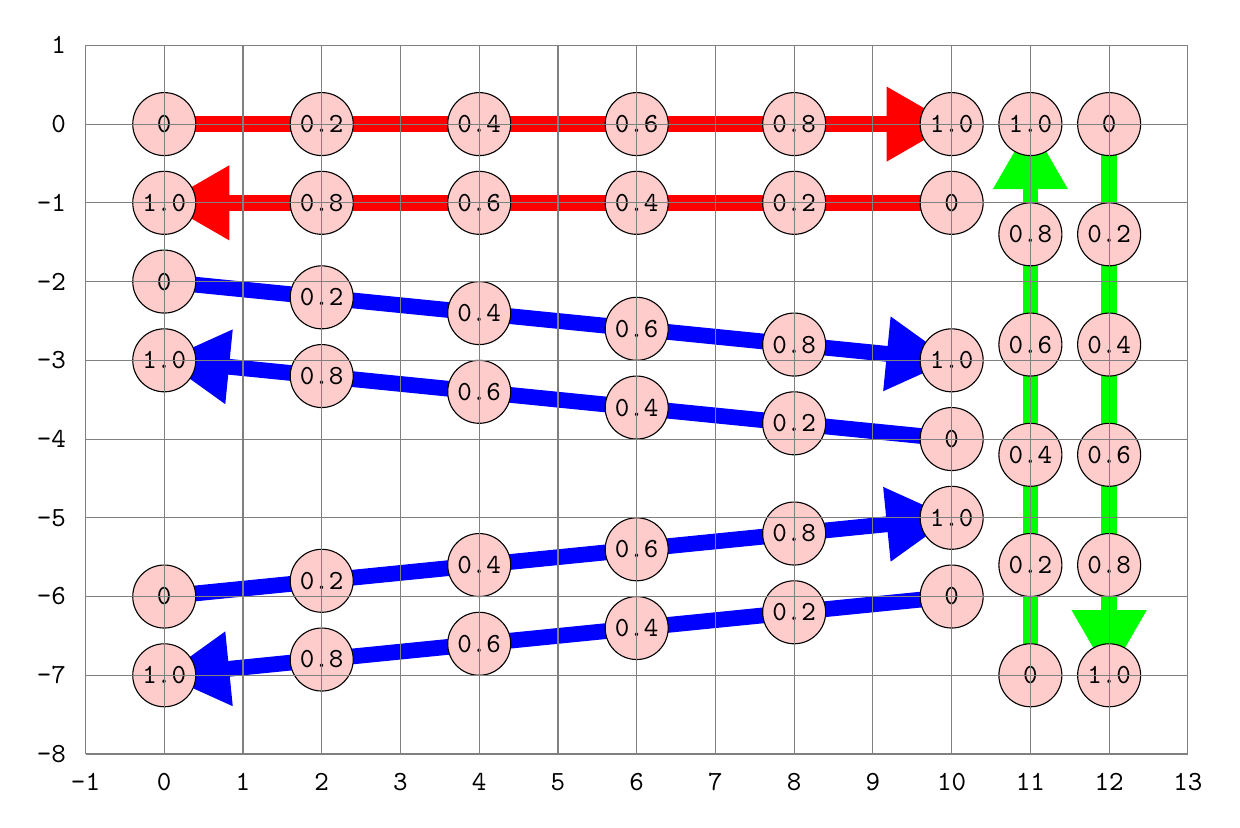
\begin{tikzpicture}
\draw[line width=0.2cm,red,->,>=triangle 60] (0,0) -- (10,0);
\fill[red] (0, 0) circle (0);

\draw[red] (0, 0)
circle (0.0);
\fill[red!20] (0.0, 0.0) circle (0.4);

\draw[black] (0.0, 0.0)
circle (0.4);
\draw (0.0, 0.0) node[color=black] {{\texttt{0}}};\fill[red!20] (2.0, 0.0) circle (0.4);

\draw[black] (2.0, 0.0)
circle (0.4);
\draw (2.0, 0.0) node[color=black] {{\texttt{0.2}}};\fill[red!20] (4.0, 0.0) circle (0.4);

\draw[black] (4.0, 0.0)
circle (0.4);
\draw (4.0, 0.0) node[color=black] {{\texttt{0.4}}};\fill[red!20] (6.0, 0.0) circle (0.4);

\draw[black] (6.0, 0.0)
circle (0.4);
\draw (6.0, 0.0) node[color=black] {{\texttt{0.6}}};\fill[red!20] (8.0, 0.0) circle (0.4);

\draw[black] (8.0, 0.0)
circle (0.4);
\draw (8.0, 0.0) node[color=black] {{\texttt{0.8}}};\fill[red!20] (10.0, 0.0) circle (0.4);

\draw[black] (10.0, 0.0)
circle (0.4);
\draw (10.0, 0.0) node[color=black] {{\texttt{1.0}}};\draw[line width=0.2cm,red,->,>=triangle 60] (10,-1) -- (0,-1);
\fill[red] (10, -1) circle (0);

\draw[red] (10, -1)
circle (0.0);
\fill[red!20] (10.0, -1.0) circle (0.4);

\draw[black] (10.0, -1.0)
circle (0.4);
\draw (10.0, -1.0) node[color=black] {{\texttt{0}}};\fill[red!20] (8.0, -1.0) circle (0.4);

\draw[black] (8.0, -1.0)
circle (0.4);
\draw (8.0, -1.0) node[color=black] {{\texttt{0.2}}};\fill[red!20] (6.0, -1.0) circle (0.4);

\draw[black] (6.0, -1.0)
circle (0.4);
\draw (6.0, -1.0) node[color=black] {{\texttt{0.4}}};\fill[red!20] (4.0, -1.0) circle (0.4);

\draw[black] (4.0, -1.0)
circle (0.4);
\draw (4.0, -1.0) node[color=black] {{\texttt{0.6}}};\fill[red!20] (2.0, -1.0) circle (0.4);

\draw[black] (2.0, -1.0)
circle (0.4);
\draw (2.0, -1.0) node[color=black] {{\texttt{0.8}}};\fill[red!20] (0.0, -1.0) circle (0.4);

\draw[black] (0.0, -1.0)
circle (0.4);
\draw (0.0, -1.0) node[color=black] {{\texttt{1.0}}};\draw[line width=0.2cm,blue,->,>=triangle 60] (0,-2) -- (10,-3);
\fill[blue] (0, -2) circle (0);

\draw[blue] (0, -2)
circle (0.0);
\fill[red!20] (0.0, -2.0) circle (0.4);

\draw[black] (0.0, -2.0)
circle (0.4);
\draw (0.0, -2.0) node[color=black] {{\texttt{0}}};\fill[red!20] (2.0, -2.2) circle (0.4);

\draw[black] (2.0, -2.2)
circle (0.4);
\draw (2.0, -2.2) node[color=black] {{\texttt{0.2}}};\fill[red!20] (4.0, -2.4) circle (0.4);

\draw[black] (4.0, -2.4)
circle (0.4);
\draw (4.0, -2.4) node[color=black] {{\texttt{0.4}}};\fill[red!20] (6.0, -2.6) circle (0.4);

\draw[black] (6.0, -2.6)
circle (0.4);
\draw (6.0, -2.6) node[color=black] {{\texttt{0.6}}};\fill[red!20] (8.0, -2.8) circle (0.4);

\draw[black] (8.0, -2.8)
circle (0.4);
\draw (8.0, -2.8) node[color=black] {{\texttt{0.8}}};\fill[red!20] (10.0, -3.0) circle (0.4);

\draw[black] (10.0, -3.0)
circle (0.4);
\draw (10.0, -3.0) node[color=black] {{\texttt{1.0}}};\draw[line width=0.2cm,blue,->,>=triangle 60] (10,-4) -- (0,-3);
\fill[blue] (10, -4) circle (0);

\draw[blue] (10, -4)
circle (0.0);
\fill[red!20] (10.0, -4.0) circle (0.4);

\draw[black] (10.0, -4.0)
circle (0.4);
\draw (10.0, -4.0) node[color=black] {{\texttt{0}}};\fill[red!20] (8.0, -3.8) circle (0.4);

\draw[black] (8.0, -3.8)
circle (0.4);
\draw (8.0, -3.8) node[color=black] {{\texttt{0.2}}};\fill[red!20] (6.0, -3.6) circle (0.4);

\draw[black] (6.0, -3.6)
circle (0.4);
\draw (6.0, -3.6) node[color=black] {{\texttt{0.4}}};\fill[red!20] (4.0, -3.4) circle (0.4);

\draw[black] (4.0, -3.4)
circle (0.4);
\draw (4.0, -3.4) node[color=black] {{\texttt{0.6}}};\fill[red!20] (2.0, -3.2) circle (0.4);

\draw[black] (2.0, -3.2)
circle (0.4);
\draw (2.0, -3.2) node[color=black] {{\texttt{0.8}}};\fill[red!20] (0.0, -3.0) circle (0.4);

\draw[black] (0.0, -3.0)
circle (0.4);
\draw (0.0, -3.0) node[color=black] {{\texttt{1.0}}};\draw[line width=0.2cm,blue,->,>=triangle 60] (0,-6) -- (10,-5);
\fill[blue] (0, -6) circle (0);

\draw[blue] (0, -6)
circle (0.0);
\fill[red!20] (0.0, -6.0) circle (0.4);

\draw[black] (0.0, -6.0)
circle (0.4);
\draw (0.0, -6.0) node[color=black] {{\texttt{0}}};\fill[red!20] (2.0, -5.8) circle (0.4);

\draw[black] (2.0, -5.8)
circle (0.4);
\draw (2.0, -5.8) node[color=black] {{\texttt{0.2}}};\fill[red!20] (4.0, -5.6) circle (0.4);

\draw[black] (4.0, -5.6)
circle (0.4);
\draw (4.0, -5.6) node[color=black] {{\texttt{0.4}}};\fill[red!20] (6.0, -5.4) circle (0.4);

\draw[black] (6.0, -5.4)
circle (0.4);
\draw (6.0, -5.4) node[color=black] {{\texttt{0.6}}};\fill[red!20] (8.0, -5.2) circle (0.4);

\draw[black] (8.0, -5.2)
circle (0.4);
\draw (8.0, -5.2) node[color=black] {{\texttt{0.8}}};\fill[red!20] (10.0, -5.0) circle (0.4);

\draw[black] (10.0, -5.0)
circle (0.4);
\draw (10.0, -5.0) node[color=black] {{\texttt{1.0}}};\draw[line width=0.2cm,blue,->,>=triangle 60] (10,-6) -- (0,-7);
\fill[blue] (10, -6) circle (0);

\draw[blue] (10, -6)
circle (0.0);
\fill[red!20] (10.0, -6.0) circle (0.4);

\draw[black] (10.0, -6.0)
circle (0.4);
\draw (10.0, -6.0) node[color=black] {{\texttt{0}}};\fill[red!20] (8.0, -6.2) circle (0.4);

\draw[black] (8.0, -6.2)
circle (0.4);
\draw (8.0, -6.2) node[color=black] {{\texttt{0.2}}};\fill[red!20] (6.0, -6.4) circle (0.4);

\draw[black] (6.0, -6.4)
circle (0.4);
\draw (6.0, -6.4) node[color=black] {{\texttt{0.4}}};\fill[red!20] (4.0, -6.6) circle (0.4);

\draw[black] (4.0, -6.6)
circle (0.4);
\draw (4.0, -6.6) node[color=black] {{\texttt{0.6}}};\fill[red!20] (2.0, -6.8) circle (0.4);

\draw[black] (2.0, -6.8)
circle (0.4);
\draw (2.0, -6.8) node[color=black] {{\texttt{0.8}}};\fill[red!20] (0.0, -7.0) circle (0.4);

\draw[black] (0.0, -7.0)
circle (0.4);
\draw (0.0, -7.0) node[color=black] {{\texttt{1.0}}};\draw[line width=0.2cm,green,->,>=triangle 60] (11,-7) -- (11,0);
\fill[green] (11, -7) circle (0);

\draw[green] (11, -7)
circle (0.0);
\fill[red!20] (11.0, -7.0) circle (0.4);

\draw[black] (11.0, -7.0)
circle (0.4);
\draw (11.0, -7.0) node[color=black] {{\texttt{0}}};\fill[red!20] (11.0, -5.6) circle (0.4);

\draw[black] (11.0, -5.6)
circle (0.4);
\draw (11.0, -5.6) node[color=black] {{\texttt{0.2}}};\fill[red!20] (11.0, -4.2) circle (0.4);

\draw[black] (11.0, -4.2)
circle (0.4);
\draw (11.0, -4.2) node[color=black] {{\texttt{0.4}}};\fill[red!20] (11.0, -2.8) circle (0.4);

\draw[black] (11.0, -2.8)
circle (0.4);
\draw (11.0, -2.8) node[color=black] {{\texttt{0.6}}};\fill[red!20] (11.0, -1.4) circle (0.4);

\draw[black] (11.0, -1.4)
circle (0.4);
\draw (11.0, -1.4) node[color=black] {{\texttt{0.8}}};\fill[red!20] (11.0, 0.0) circle (0.4);

\draw[black] (11.0, 0.0)
circle (0.4);
\draw (11.0, 0.0) node[color=black] {{\texttt{1.0}}};\draw[line width=0.2cm,green,->,>=triangle 60] (12,0) -- (12,-7);
\fill[green] (12, 0) circle (0);

\draw[green] (12, 0)
circle (0.0);
\fill[red!20] (12.0, 0.0) circle (0.4);

\draw[black] (12.0, 0.0)
circle (0.4);
\draw (12.0, 0.0) node[color=black] {{\texttt{0}}};\fill[red!20] (12.0, -1.4) circle (0.4);

\draw[black] (12.0, -1.4)
circle (0.4);
\draw (12.0, -1.4) node[color=black] {{\texttt{0.2}}};\fill[red!20] (12.0, -2.8) circle (0.4);

\draw[black] (12.0, -2.8)
circle (0.4);
\draw (12.0, -2.8) node[color=black] {{\texttt{0.4}}};\fill[red!20] (12.0, -4.2) circle (0.4);

\draw[black] (12.0, -4.2)
circle (0.4);
\draw (12.0, -4.2) node[color=black] {{\texttt{0.6}}};\fill[red!20] (12.0, -5.6) circle (0.4);

\draw[black] (12.0, -5.6)
circle (0.4);
\draw (12.0, -5.6) node[color=black] {{\texttt{0.8}}};\fill[red!20] (12.0, -7.0) circle (0.4);

\draw[black] (12.0, -7.0)
circle (0.4);
\draw (12.0, -7.0) node[color=black] {{\texttt{1.0}}};\draw[gray] (-1.0,-8.0) -- (-1.0,1);
\draw[gray] (0.0,-8.0) -- (0.0,1);
\draw[gray] (1.0,-8.0) -- (1.0,1);
\draw[gray] (2.0,-8.0) -- (2.0,1);
\draw[gray] (3.0,-8.0) -- (3.0,1);
\draw[gray] (4.0,-8.0) -- (4.0,1);
\draw[gray] (5.0,-8.0) -- (5.0,1);
\draw[gray] (6.0,-8.0) -- (6.0,1);
\draw[gray] (7.0,-8.0) -- (7.0,1);
\draw[gray] (8.0,-8.0) -- (8.0,1);
\draw[gray] (9.0,-8.0) -- (9.0,1);
\draw[gray] (10.0,-8.0) -- (10.0,1);
\draw[gray] (11.0,-8.0) -- (11.0,1);
\draw[gray] (12.0,-8.0) -- (12.0,1);
\draw[gray] (13.0,-8.0) -- (13.0,1);
\draw[gray] (-1.0,-8.0) -- (13,-8.0);
\draw[gray] (-1.0,-7.0) -- (13,-7.0);
\draw[gray] (-1.0,-6.0) -- (13,-6.0);
\draw[gray] (-1.0,-5.0) -- (13,-5.0);
\draw[gray] (-1.0,-4.0) -- (13,-4.0);
\draw[gray] (-1.0,-3.0) -- (13,-3.0);
\draw[gray] (-1.0,-2.0) -- (13,-2.0);
\draw[gray] (-1.0,-1.0) -- (13,-1.0);
\draw[gray] (-1.0,0.0) -- (13,0.0);
\draw[gray] (-1.0,1.0) -- (13,1.0);
\draw(-1, -8) node [font=\ttfamily, label=below:{\texttt{-1}}] {};
\draw(0, -8) node [font=\ttfamily, label=below:{\texttt{0}}] {};
\draw(1, -8) node [font=\ttfamily, label=below:{\texttt{1}}] {};
\draw(2, -8) node [font=\ttfamily, label=below:{\texttt{2}}] {};
\draw(3, -8) node [font=\ttfamily, label=below:{\texttt{3}}] {};
\draw(4, -8) node [font=\ttfamily, label=below:{\texttt{4}}] {};
\draw(5, -8) node [font=\ttfamily, label=below:{\texttt{5}}] {};
\draw(6, -8) node [font=\ttfamily, label=below:{\texttt{6}}] {};
\draw(7, -8) node [font=\ttfamily, label=below:{\texttt{7}}] {};
\draw(8, -8) node [font=\ttfamily, label=below:{\texttt{8}}] {};
\draw(9, -8) node [font=\ttfamily, label=below:{\texttt{9}}] {};
\draw(10, -8) node [font=\ttfamily, label=below:{\texttt{10}}] {};
\draw(11, -8) node [font=\ttfamily, label=below:{\texttt{11}}] {};
\draw(12, -8) node [font=\ttfamily, label=below:{\texttt{12}}] {};
\draw(13, -8) node [font=\ttfamily, label=below:{\texttt{13}}] {};
\draw(-1, -8) node [font=\ttfamily, label=left:{\texttt{-8}}] {};
\draw(-1, -7) node [font=\ttfamily, label=left:{\texttt{-7}}] {};
\draw(-1, -6) node [font=\ttfamily, label=left:{\texttt{-6}}] {};
\draw(-1, -5) node [font=\ttfamily, label=left:{\texttt{-5}}] {};
\draw(-1, -4) node [font=\ttfamily, label=left:{\texttt{-4}}] {};
\draw(-1, -3) node [font=\ttfamily, label=left:{\texttt{-3}}] {};
\draw(-1, -2) node [font=\ttfamily, label=left:{\texttt{-2}}] {};
\draw(-1, -1) node [font=\ttfamily, label=left:{\texttt{-1}}] {};
\draw(-1, 0) node [font=\ttfamily, label=left:{\texttt{0}}] {};
\draw(-1, 1) node [font=\ttfamily, label=left:{\texttt{1}}] {};
\end{tikzpicture}

\end{center}

\end{document}
